% arara: pdflatex
% arara: pdflatex
% arara: pdflatex
% arara: pdflatex
% ----------------------------------------------------------------------------
% the XSIM package
% 
%   eXercise Sheets IMproved
% 
% ----------------------------------------------------------------------------
% Clemens Niederberger
% Web:    https://github.com/cgnieder/xsim
% E-Mail: contact@mychemistry.eu
% ----------------------------------------------------------------------------
% Copyright 2017 Clemens Niederberger
% 
% This work may be distributed and/or modified under the
% conditions of the LaTeX Project Public License, either version 1.3
% of this license or (at your option) any later version.
% The latest version of this license is in
%   http://www.latex-project.org/lppl.txt
% and version 1.3 or later is part of all distributions of LaTeX
% version 2005/12/01 or later.
% 
% This work has the LPPL maintenance status `maintained'.
% 
% The Current Maintainer of this work is Clemens Niederberger.
% ----------------------------------------------------------------------------
% If you have any ideas, questions, suggestions or bugs to report, please
% feel free to contact me.
% ----------------------------------------------------------------------------
\documentclass{xsim-manual}

\begin{filecontents}{\jobname.bib}
@online{texsx:romannumeral,
  author = {Bruno Le Floch} ,
  title = {Cunning (La)TeX tricks} ,
  urldate = {2017-03-02} ,
  url = {http://tex.stackexchange.com/a/19769/}
}
\end{filecontents}
\addbibresource{\jobname.bib}

\begin{document}

\section{Licence, Requirements and \textsc{README}}
\license

\xsim\ loads the packages \pkg{expl3}~\cite{bnd:l3kernel},
\pkg{xparse}~\cite{bnd:l3packages}, \pkg{etoolbox}~\cite{pkg:etoolbox},
\pkg{booktabs}~\cite{pkg:booktabs} and
\pkg{translations}~\cite{pkg:translations}.  All of these packages are present
on a modern and up to date \TeX\ distribution such as \TeX~Live or MiK\TeX\ so
no further action should be needed.

\section{Motivation and Background}

It has been quite a while since I first published
\pkg{exsheets}~\cite{pkg:exsheets} in Juni 2012.  Since then it has gained a
user base and a little bit of popularity as the number of questions on tex.sx
shows (98~at the time of writing).  User questions, bug reports and feature
requests improved it over the time.  It still has a version number starting
with a zero, though, which in my versioning system means I still consider it
experimental.

This is due to several facts.  It lacks a few features which I consider
essential for a full version~1.  For one thing it is not possible to have
several kinds of exercises numbered independently.  Using verbatim material
such as listings inside exercises and solutions is not possible and the
current workaround isn't that ideal either.  One request which dates back
quite a while now was to have different types of points to exercises\ldots

All of those aren't easy to add due to the way \pkg{exsheets} is implemented
right now. As a consequence I wanted to re-implement \pkg{exsheets} for a long
time.  This is what lead to \xsim.  Internally the package works completely
different. It will be the official successor of \pkg{exsheets} which is now
considered obsolete and will only receive bugfix releases any more.

\section{Package Options}\label{sec:package-options}
\xsim\ has two package options:
\begin{options}
  \opt{verbose}
    Writes extensive information about what \xsim\ is doing into the log
    file.
  \opt{final}
    If used the exercise and solution environments will not rewrite the
    environment body files.
\end{options}

Those options are used the usual way as package option
\begin{sourcecode}
  \usepackage[verbose]{xsim}
\end{sourcecode}
or as global option
\begin{sourcecode}
  \documentclass[verbose]{article}
\end{sourcecode}
or via the setup command:
\begin{commands}
  \command{xsimsetup}[\marg{options}]
    Set up \xsim's two package options and all other options described at
    other places in the manual.
\end{commands}

\section{How to Read the Manual}\label{sec:how-read-manual}

\subsection{Nomenclature}

Throughout this manual certain terms are used.  This section explains their
meaning in this manual.

\acuseall
\printacronyms[heading=none]

\subsection{Setting Options}
Apart from the package options already described in
section~\vref{sec:package-options} \xsim\ has further options. Those can be
\enquote{toplevel} options or options belonging to a module.
\begin{options}
  \keyval*{toplevel}{value}
    A toplevel option.
  \keyval*{sublebel}{value}\Module*{module}
    A sublevel option belonging to the module \module*{module}
\end{options}
Both kinds of options are set with \cs{xsimsetup}:
\begin{sourcecode}
  \xsimsetup{
    toplevel = {value} ,
    module/sublevel = {value}
  }
\end{sourcecode}

\subsection{Command descriptions}

Some commands do have a \expandablesymbol\ symbol printed next to their
names.  This indicates that the command is expandable, \ie, it is usable in an
\cs*{edef} or \cs*{write} context and will expand according to its
description.  All other commands are engine protected, \ie, in the sense of
\eTeX's \cs*{protected}.

Some command name descriptions end with \cs*{\TF}.
\begin{commands}
  \command*{SomeCommand\TF}[\meta{arguments}\marg{true}\marg{false}]
    A command with maybe some arguments and ending with the two arguments
    \meta{true} and \meta{false}.
\end{commands}
This means two things: the command is a conditional which tests something and
depending on the outcome of the test leaves either the \meta{true} argument
(\code{T}) or the \meta{false} argument (\code{F}) in the input stream.  It
also means to additional commands exist:
\begin{commands}
  \command*{SomeCommandT}[\meta{arguments}\marg{true}]
    The same as \cs*{SomeCommandTF} but only with the \meta{true} argument and
    no \meta{false} argument.
  \command*{SomeCommandF}[\meta{arguments}\marg{false}]
    The same as \cs*{SomeCommandTF} but only with the \meta{false} argument and
    no \meta{true} argument.
\end{commands}


\section{Exercises and Solutions}

\subsection{The Environments}

\begin{environments}
  \environment{exercise}[\oarg{\acsp*{prop}}]
    Input and typeset an exercise.  See section~\vref{sec:exercise-properties}
    for details on exercise \acsp*{prop}.
  \environment{solution}[\oarg{options}]
    Input and typeset the solution to the exercise of the previous
    \env{exercise} environment.  See section~\vref{sec:printing-solutions} for
    details on options of solutions.
\end{environments}

\begin{example}
  \begin{exercise}
    A first example for an exercise.
  \end{exercise}
  \begin{solution}
    A first example for a solution.
  \end{solution}
\end{example}

As can be seen in the example a solution is not printed with the default
setup.  This can be changed using the following option.
\begin{options}
  \keybool{print}\Module{solution}\Default{false}
    Set if solutions are printed or or not.
\end{options}

The option (belonging to the module \module*{solution}) can either be set
locally as option to the \env{solution} environment
\begin{sourcecode}
  \begin{solution}[print=true]
    A first example for a solution.
  \end{solution}
\end{sourcecode}
or with the setup command for all following solutions:
\begin{sourcecode}
  \xsimsetup{
    solution/print = true
  }
\end{sourcecode}

There is an completely analoguous option for the \env{exercise} environment:
\begin{options}
  \keybool{print}\Module{exercise}\Default{true}
    Set if exercises are printed or or not.
\end{options}
See also section~\vref{sec:using-printing}.

\section{How the Exercise Environments Work}
Both enviroments write the contents of their bodies verbatim to external files
following a certain naming structure:
\begin{itemize}
  \item
  \code{\meta{jobname}-\meta{type}-\meta{id}-exercise|solution-body.tex} 
\end{itemize}
The name starts with the name of the job (which is the name of the document
itself) followed by type and id of the corresponding exercise and then
followed by the environment type.  For example both enviroments from the first
example have been written to files named
\begin{itemize}
  \item \verbcode+xsim_manual-exercise-1-exercise-body.tex+ and
  \item \verbcode+xsim_manual-exercise-1-solution-body.tex+, respectively.
\end{itemize}
Details on the \meta{type} of an exercise will be given in
section~\vref{sec:new-exercise-types}.  \emph{The \meta{id} of an exercise is
  a positive integer unique to each exercise environment regardless if the
  exercise is being printed or used at all.}

These external files are input when the respective exercise or solution is
printed.  An advantage of using external files is that \emph{verbatim material
  is allowed} inside the environments.  Each of those files contains some
information about itself and where and why it was generated\footnote{In this
  example the sourcecode line number is misleading as the example where the
  file was generated itself was an external file where the \env{exercise}
  environment indeed \emph{was} on line~1.}:

\inputsourcecode{exercises/xsim_manual-exercise-1-exercise-body.tex}

Arguably one downside of the approach using external files for each exercise
and its solution is that your project folder will be cluttered with files.  In
order to deal with this somehow \xsim\ offers the following option:
\begin{options}
  \keyval{path}{path name}\Default
    With this option a subfolder or path within the main project folder can be
    given.  Exercises will be written to and included from this path.
    \emph{The path must exist on your system before you can use it!} This
    document uses \keyis{path}{exercises}.
\end{options}

\section{New Exercise Types}\label{sec:new-exercise-types}

It is easy to define new exercise environments together with a corresponding
solution environment using the following command:
\begin{commands}
  \command{DeclareExerciseType}[\marg{type}\marg{parameters}]
    Declare a new exercise type analoguous to the \env{exercise} and
    \env{solution} environments.
\end{commands}

The existing environment pair has been defined as follows:
\begin{sourcecode}
  \DeclareExerciseType{exercise}{
    exercise-env      = exercise ,
    solution-env      = solution ,
    exercise-name     = \XSIMtranslate{exercise} ,
    solution-name     = \XSIMtranslate{solution} ,
    exercise-template = default ,
    solution-template = default
  }
\end{sourcecode}

The above already is an example for almost all parameters that can (and often
must) be set.  Here is the complete list:
\begin{parameters}
  \paraval{exercise-env}{exercise environment name}
    The name for the environment used for the exercises of type \meta{type}.
    \emph{This parameter must be set.}
  \paraval{solution-env}{solution environment name}
    The name for the environment used for the solutions of type \meta{type}.
    \emph{This parameter must be set.}
  \paraval{exercise-name}{exercise name}
    The name of the exercises of type \meta{type} -- used for typesetting.
    \emph{This parameter must be set.}
  \paraval{solution-name}{solution name}
    The name of the solutions of type \meta{type} -- used for typesetting.
    \emph{This parameter must be set.}
  \paraval{exercise-template}{exercise template}
    The template used for typesetting the exercises of type \meta{type}.
    \emph{This parameter must be set.} See section~\vref{sec:styl-exerc-templ}
    for details on templates.
  \paraval{solution-template}{solution template}
    The template used for typesetting the exercises of type \meta{type}.
    \emph{This parameter must be set.} See section~\vref{sec:styl-exerc-templ}
    for details on templates.
  \paraval{counter}{counter name}
    The counter used for the exercises of type \meta{type}.  If not explicitly
    set the counter with the same name as \parameter{exercise-env} is used.
    Otherwise the specified counter is used.  This enables to have different
    types of exercises sharing a common counter.
  \paraval{counter}{integer}
    An internal parameter that is used to keep track of the number of
    exercises of a type.
\end{parameters}

It is possible to change some of the parameters after an exercise type has
been defined.  Those include \parameter{exercise-name},
\parameter{solution-name}, \parameter{exercise-template},
\parameter{solution-template}, and \parameter{counter}:
\begin{commands}
  \command{SetExerciseParameter}[\marg{type}\marg{parameter}\marg{value}]
    Usable to set a single parameter to a new value.
  \command{SetExerciseParameters}[\marg{type}\marg{parameters}]
    Set several parameters at once. \meta{parameters} is a csv list of
    key/value pairs.
\end{commands}
If you try to set an already set but fixed parameter like
\parameter{exercise-env} a warning will be written to the log file.  If you
set \parameter{counter} to another value you must make sure that the new value
is a valid and defined counter.

\section{Exercise Properties}\label{sec:exercise-properties}

\subsection{Predefined Properties}

Exercise like the \env{exercise} environment and possibly others defined with
\cs{DeclareExerciseType} have a number of predefined \acsp*{prop}:
\begin{properties}
  \propval{id}{integer}
    Holds the internal id of an exercise.  \emph{Cannot be set by the user}.
  \propval{ID}{text}
    Holds the user id of an exercise if defined.  Otherwise it is equal to
    \property{id}.
  \propval{counter}{integer}
    Holds the counter value of an exercise.  \emph{Cannot be set by the
      user}.
  \propval{subtitle}{text}
    Holds the subtitle of an exercise.
  \propval{points}{number}
    Holds the reachable points of an exercise.
  \propval{bonus-points}{number}
    Holds the reachable bonus-points of an exercise.
  \propbool{print}
    Holds the print boolean of an exercise.
  \propbool{use}
    Holds the usage boolean of an exercise.
  \propval{tags}{csv list of tags}
    Holds the list of tags the exercise should be associated with.
  \propval{topics}{csv list of topics}
    Holds the list of topics the exercise should be associated with.
\end{properties}

Some of these \acsp*{prop} are fixed and cannot be set by the user.  Those
include \property{id} and \property{counter}.  The others can be set using the
optional argument of the exercise environment.

\begin{example}
  \begin{exercise}[subtitle={This is a subtitle}]
    An exercise where some properties have been set.
  \end{exercise}
\end{example}

\subsection{Declaring Own Properties}

\xsim\ offers the possibility to declare additional exercise properties:
\begin{commands}
  \command{DeclareExerciseProperty}[\sarg\marg{property}]
    Declares the property \meta{property}.  If used with the optional star a
    unique property is defined which means that each exercise must have a
    property value distinct from all other exercises.
  \command{DeclareExercisePropertyAlias}[\marg{property 1}\marg{property 2}]
    Declares \meta{property 1} to be an alias of \meta{property 2}.  This
    means that each time \meta{property 2} is set \meta{property 1} will be
    set to the same value \emph{unless} it has been set already.  As an
    example: property \property{ID} is an alias of property \property{id}.
\end{commands}

This is better demonstrated with an example:
\begin{example}
  \begin{exercise}
    \lipsum[4] % from package `lipsum'
    \verb+\GetExerciseProperty{id}+: \GetExerciseProperty{id} \par
    \verb+\GetExerciseAliasProperty{ID}+: \GetExerciseAliasProperty{ID} \par
    \verb+\GetExerciseProperty{ID}+: \GetExerciseProperty{ID}
  \end{exercise}
  \begin{exercise}[ID=foo-bar]
    \lipsum[4]
    \verb+\GetExerciseProperty{id}+: \GetExerciseProperty{id} \par
    \verb+\GetExerciseAliasProperty{ID}+: \GetExerciseAliasProperty{ID} \par
    \verb+\GetExerciseProperty{ID}+: \GetExerciseProperty{ID}
  \end{exercise}
\end{example}

The power of properties will get more clear when reading
section~\vref{sec:styl-exerc-templ} about templates.

\subsection{A Special Kind of Property: Exercise Goals}\label{sec:goals}

Exercise goals are a generic concept in \xsim\ for exercise properties like
\property{points} or \property{bonus-points}.  Those are properties which can
(only) get a decimal number as value the sum of which is calculated and
available (after a compilation) throughout the document.
\begin{commands}
  \command{DeclareExerciseGoal}[\marg{goal}]
    Declare a new exercise goal named \meta{goal} and also a property called
    \meta{goal}.
  \command{TotalExerciseTypeGoal}[\marg{type}\marg{goal}\marg{singular}\marg{plural}]
    Get the sum of goal \meta{goal} for all exercises of type \meta{type}.
    \meta{singular} andf \meta{plural} are placed after the sum in the input
    stream depending on whether the sum equals~$1$ or not.
  \command{TotalExerciseGoal}[\marg{goal}\marg{singular}\marg{plural}]
    Get the sum of goal \meta{goal} for all exercises. \meta{singular} andf
    \meta{plural} are placed after the sum in the input stream depending on
    whether the sum equals~$1$ or not.
  \command{printpoints}[\marg{type}]
    Print the sum of points for all exercises of type \meta{type} followed by
    an appropriate translation of the words \enquote{point} or
    \enquote{points}, respectively\footnote{See section~\vref{sec:exerc-transl}
      for details on the definition and usage of language dependent words.}.
    Defined in terms of \cs{TotalExerciseTypeGoal}.
  \command{printtotalpoints}
    Print the sum of points for all exercises followed by an appropriate
    translation of the words \enquote{point} or \enquote{points},
    respectivaly.  Defined in terms of \cs{TotalExerciseGoal}.
  \command{printbonus}[\marg{type}]
    Print the sum of bonus points for all exercises of type \meta{type}
    followed by an appropriate translation of the words \enquote{point} or
    \enquote{points}, respectivaly.  Defined in terms of
    \cs{TotalExerciseTypeGoal}.
  \command{printtotalbonus}
    Print the sum of bonus points for all exercises followed by an appropriate
    translation of the words \enquote{point} or \enquote{points},
    respectivaly.  Defined in terms of \cs{TotalExerciseGoal}.
\end{commands}

The two existing goals are defined with
\begin{sourcecode}
  \DeclareExerciseGoal{points}
  \DeclareExerciseGoal{bonus-points}
\end{sourcecode}

When goal values are printed the decimal number is fed to a function which can
be changed using the following option:
\begin{options}
  \keyval{goal-print}{code}\Default{\#1}
    How to format goal values.  Use \code{\#1} to refer to the actual number.
\end{options}

\subsection{A Special Kind of Property: Exercise Tags}\label{sec:tags}

Exercise tags are a generic concept in \xsim\ for exercise properties like
\property{tags} or \property{topics}.  Those are properties which can (only)
get a csv list of strings as value.  Those strings can be used to selectively
use exercises.  See section~\vref{sec:using-printing} for details on
\emph{usage} of exercises and the difference to \emph{printing} an exercise
and how to use exercise tags for selection.
\begin{commands}
  \command{DeclareExerciseTagging}{tag}
    This defines an exercise tagging group name \meta{tag}.  It also defines a
    property named \meta{tag}.  In addition to options are defines: and option
    named \code{\meta{tag}} which can be used for selection and an boolean
    option \code{\meta{tag}/ignore-untagged}.
\end{commands}
The two existing tagging groups have been defined and preset with the
following code:
\begin{sourcecode}
  \DeclareExerciseTagging{tags}
  \DeclareExerciseTagging{topics}
  \xsimsetup{tags/ingore-untagged=false}
\end{sourcecode}
this means that these options are available:
\begin{options}
  \keyval{tags}{csv list of tags}
    Choose the set of tags whose associated exercises should be printed.
  \keyval{topics}{csv list of topics}
    Choose the set of tags whose associated exercises should be printed.
  \keybool{ignore-tagging}\Module{tags}\Default{false}
    If set to true exercises with no tags will be printed even if tags have
    been chosen with the option \option{tags}.
  \keybool{ignore-tagging}\Module{topics}\Default{true}
    If set to true exercises with no topics will be printed even if tags have
    been chosen with the option \option{tags}.
\end{options}

\section{Using and Printing an Exercise}\label{sec:using-printing}

\subsection{What the Environments do}

When an exercise is started with \environ{exercise} (or other environments
defined through \cs{DeclareExerciseType}) then different things happen
depending on different settings:
\begin{itemize}
  \item If the \emph{insert mode} is active nothing happens, see
    section~\vref{sec:collecting-exercises} for details on this.
  \item Else the id integer is incremented.
  \item If the exercise is \emph{used} the corresponding counter is stepped
    and the exercise is added to the \enquote{use list}.  The properties
    \property{counter} and \property{use} are updated accordingly.
  \item If an exercise is printed then it is also used. An exercise that isn't
    used cannot be printed.  Being printed means two things: being added to
    the \enquote{print list} and being typeset at the position where the
    exercise is placed in the source file.  If an exercise is \emph{not
      printed but used} it means that the counter will be stepped.  This can
    be useful for creating an exercise sheet only containing the solutions for
    some exercises.
  \item If an exercise is printed certain hooks and template code is inserted
    around the environment body.
\end{itemize}

\begin{example}[outside]
  \begin{exercise}[print=false]
    This exercise will not be printed but the exercise counter will be
    incremented nonetheless. Its solution will be printed in the list of
    solutions.
  \end{exercise}
  \begin{solution}
    The solution of the exercise that has not been printed.
  \end{solution}
\end{example}

The schematic structure of an exercise is shown in
figure~\vref{fig:schematic-structure}.

\begin{figure}
  \centering
  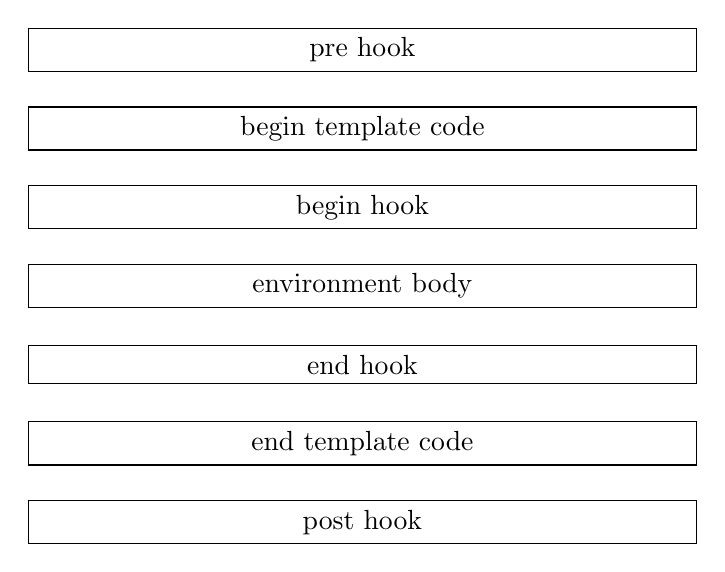
\begin{tikzpicture}
    \node[draw,minimum width=.7\linewidth] at (0,0)  {pre hook};
    \node[draw,minimum width=.7\linewidth] at (0,-1) {begin template code};
    \node[draw,minimum width=.7\linewidth] at (0,-2) {begin hook};
    \node[draw,minimum width=.7\linewidth] at (0,-3) {environment body};
    \node[draw,minimum width=.7\linewidth] at (0,-4) {end hook};
    \node[draw,minimum width=.7\linewidth] at (0,-5) {end template code};
    \node[draw,minimum width=.7\linewidth] at (0,-6) {post hook};
  \end{tikzpicture}
  \caption{Schematic structure of an exercise or solution.}\label{fig:schematic-structure} 
\end{figure}

\subsection{Environment Options \& Hooks}\label{sec:environment-options-hooks}

For each exercise type there are the following options for both environments,
the environments' names are the module names for the options (here using the
\enquote{exercise} type):
\begin{options}
  \keybool{print}\Module{exercise}\Default{true}
    Determines if exercises of type \enquote{exercise} are printed.
  \keybool{use}\Module{exercise}\Default{true}
    Determines if exercises of type \enquote{exercise} are used.
  \keyval{pre-hook}{code}\Module{exercise}\Default
    The code for the \emph{pre exercise hook} for exercises of the type
    \enquote{exercise}.
  \keyval{begin-hook}{code}\Module{exercise}\Default
    The code for the \emph{begin exercise hook} for exercises of the type
    \enquote{exercise}.
  \keyval{end-hook}{code}\Module{exercise}\Default
    The code for the \emph{end exercise hook} for exercises of the type
    \enquote{exercise}.
  \keyval{post-hook}{code}\Module{exercise}\Default
    The code for the \emph{post exercise hook} for exercises of the type
    \enquote{exercise}.
  \keybool{print}\Module{solution}\Default{false}
    Determines if solutions of type \enquote{exercise} are printed.
  \keyval{pre-hook}{code}\Module{solution}\Default
    The code for the \emph{pre solution hook} for solutions of the type
    \enquote{exercise}.
  \keyval{begin-hook}{code}\Module{solution}\Default
    The code for the \emph{begin solution hook} for solutions of the type
    \enquote{exercise}.
  \keyval{end-hook}{code}\Module{solution}\Default
    The code for the \emph{end solution hook} for solutions of the type
    \enquote{exercise}.
  \keyval{post-hook}{code}\Module{solution}\Default
    The code for the \emph{post solution hook} for solutions of the type
    \enquote{exercise}.
\end{options}

\section{Collecting Exercises}\label{sec:collecting-exercises}

\xsim\ knows the concept of \enquote{exercise collections}.  A collection must
be declared in the preamble.  Using a pair of commands explained below
exercises between those commands are added to the corresponding collection but
not printed.  After a collection is completed the collection can be printed as
often as needed.
\begin{commands}
  \command{DeclareExerciseCollection}[\marg{collection name}]
    Define a new collection \meta{collection name} in the document preamble.
  \command{collectexercisestype}[\marg{collection name}\marg{exercise type}]
    Opens the collection \meta{collection name} which now collects all
    exercises of type \meta{exercise type} until the collection is closed with
    \cs{collectexercisesstop}.  Collections of other types are not collected.
  \command{collectexercises}[\marg{collection name}]
    Opens the collection \meta{collection name} which now collects all
    exercises until the collection is closed with \cs{collectexercisesstop}.
  \command{collectexercisesstop}[\marg{collection name}]
    Closes the collection \meta{collection name}.
  \command{printcollection}[\oarg{options}\marg{collection name}]
    Prints the collection \meta{collection name}, \ie, all exercises collected
    earlier.  This command cannot be used before the corresponding collection
    has been closed correctly.
\end{commands}

% TODO: options

The usage should be clear:
\begin{example}[outside]
  \collectexercises{foo}
  \begin{exercise}
    This exercise is added to the collection `foo'.
  \end{exercise}
  \collectexercisesstop{foo}
\end{example}
Once the collection is closed it can be printed:
\begin{example}
  \printcollection{foo}
\end{example}
Actually a collection can be printed \emph{before} it is opened, too.  This
needs at least two compilations, though.

You can open several collections at the same time:
\begin{sourcecode}
  \collectexercises{foo}
    ...
  \collectexercisestype{bar}{exercises}
    ...
  \collectexercisesstop{bar}
    ...
  \collectexercisesstop{foo}
\end{sourcecode}
Exercises will be added to each open collection.

There is one generic collection called \enquote{\code{all exercises}}.  As the
name already suggests it will hold all exercises.  So if you say
\begin{sourcecode}
  \printcollection{all exercises}
\end{sourcecode}
all exercises will be printed.

\begin{bewareofthedog}
  If you use \cs*{label}s inside of exercises and you print exercises more
  than once in your document (by reusing a collection for example) you will
  get
\begin{sourcecode}
  LaTeX Warning: There were multiply-defined labels.
\end{sourcecode}
  Equally if you have environments like \environ{equation} which step a
  counter inside an exercise or solution the counter will be stepped each time
  the exercise is used.
\end{bewareofthedog}

\section{Printing Solutions}\label{sec:printing-solutions}

There are two commands for printing the solutions to exercises -- one for
printing the solutions of a specific exercise type and another for printing
all solutions.
\begin{commands}
  \command{printsolutionstype}[\sarg\oarg{options}\marg{exercise type}]
    Prints the solutions of all used exercises of type \meta{exercise type}.
    The starred version only prints the solutions of all printed exercises of
    type \meta{exercise type}.
  \command{printsolutions}[\sarg\oarg{options}]
    Prints the solutions of all used exercises of all types.  The starred
    version only prints the solutions of all printed exercises of all types,
    ordered by type.
\end{commands}

\begin{example}
  \printsolutionstype{exercise}
\end{example}

The options can be diveded into two groups.  The ones in the first group
modify the layout.
\begin{options}
  \keybool{headings}\Default{true}
    If true a heading for each exercise type is inserted.
  \keyval{headings-template}{template}\Default{default}
    The heading template used when \keyis{headings}{true}.
\end{options}

The ones in the second group set conditions selecting which solutions are
printed.  If you combine those conditions a solution is printed if it meets
either of the conditions.
\begin{options}
  \keychoice{section}{\default{true},false,\meta{integer}}\Default{false}
    If you set \keyis{section}{true} only solutions of exercises of the
    current section are printed.  If you set \keyis{section}{4} only solutions
    of exercises in a section with number~$4$ are printed.
  \keychoice{chapter}{\default{true},false,\meta{integer}}\Default{false}
    If you set \keyis{chapter}{true} only solutions of exercises of the
    current chapter are printed.  If you set \keyis{chapter}{4} only solutions
    of exercises in a chapter with number~$4$ are printed.
  \keychoice{collection}{false,\meta{collection name}}\Default{false}
    If used only solutions of exercises belonging to collection
    \meta{collection name} are printed.
\end{options}

All options can also be set via \cs{xsimsetup} using the module
\module{print-solutions}.

\begin{example}
  \printsolutions[section=5,headings-template=per-section]
\end{example}

\section{Grading Tables}\label{sec:grading-tables}
When you create exercises it may not only be desirable to be able to add
points and bonus-points to a question (see section~\vref{sec:goals} about
exercise goals) but also to be able to output a grading table. \xsim\ has
built-in means for this.
\begin{commands}
  \command{gradingtable}[\oarg{options}]
    Print a grading table.
\end{commands}
Valid options for this command are
\begin{options}
  \keyval{template}{template}\Default{default}
    Choose the template used for the grading table.
  \keyval{type}{exercise type}\Default
    Choose the exercise type for which the table is printed.
\end{options}
Both option defaults can be changed with \cs{xsimsetup} setting the options
using \module{gradingtable}:
\begin{sourcecode}
  \xsimsetup{
    gradingtable/template = default*
  }
\end{sourcecode}

An example:
\begin{example}
  \gradingtable[type=exercise]
\end{example}

Or using the \enquote{\code{default*}} template:
\begin{example}
  \gradingtable[template=default*,type=exercise]
\end{example}

Available templates and how to define new ones are explained in
sections~\vref{sec:grad-table-templ} and~\vref{sec:template-examples}.  \xsim\
per default provides two templates \enquote{\code{default}} and
\enquote{\code{default*}}, the first one has a vertical layout, the second a
horizontal layout.  Both templates can be used per type like in the examples
above or for all types at once by leaving the specification \option{type}
away:
\begin{example}
  \gradingtable
\end{example}

\section{Styling the Exercises -- Templates}\label{sec:styl-exerc-templ}

\subsection{Background}
Whenever \xsim\ outputs something to be typeset it uses so-called templates
for the task.  \xsim\ knows of three different kinds of templates:
\begin{itemize}
  \item environment templates (see section~\vref{sec:envir-templ}),
  \item heading templates (see section~\vref{sec:heading-templates}) and
  \item grading table templates (see section~\vref{sec:grad-table-templ})
\end{itemize}

The most important one for the styling of the exercises are the environment
templates.  Those templates give you complete control over the look and
arrangement of an exercise.  To be able to do this \xsim\ provides a large
number of commands which can be used only inside template
definitions\footnote{The last sentence is wrong: those commands can be used
  anywhere but most of them only give useful results inside of templates.}.
Those commands are explained in the next section.  Their usage will hopefully
become clear in the examples in section~\vref{sec:template-examples}. Having
full control over the layout comes at a price: you need to be able to program
yourself in order to achieve certain layouts\footnote{I plan to incorporate
  the most common layouts -- and maybe some fancy ones, too -- in the examples
  section~\vref{sec:template-examples} but at the time of writing this is still
  up in the air.}.

\subsection{Commands for Usage in Template Definitions}
\subsubsection{Goals}
\begin{commands}
  \command{IfExerciseGoal\TF}[\marg{goal}\marg{relation and
    value}\marg{true}\marg{false}]
    Checks the sum of goal \meta{goal} against \meta{relation and value}.
  \command{IfExerciseGoalSingular\TF}[\marg{goal}\marg{true}\marg{false}]
    Checks if the value of the goal \meta{goal} of the current exercise
    equals~$1$.  This is the same as \\
    \cs{IfExerciseGoalTF}\marg{goal}\Marg{=1}\marg{true}\marg{false}.
  \command{TotalExerciseTypeGoal}[\marg{goal}\marg{type}\marg{singular}\marg{plural}]
    Print the sum of goal \meta{goal} for the exercises of type \meta{type}
    and append \meta{singular} or \meta{plural} depending on wether the sum
    equals~$1$ or not.
  \command{TotalExerciseGoal}[\marg{goal}\marg{singular}\marg{plural}]
    Print the sum of goal \meta{goal} for all exercises of all types
    and append \meta{singular} or \meta{plural} depending on wether the sum
    equals~$1$ or not.
\end{commands}

\subsubsection{Properties}
\begin{commands}
  \expandable\command{IfExercisePropertyExist\TF}[\marg{property}\marg{true}\marg{false}]
    Tests wether an exercise property with the name \meta{property} is defined.
  \command{IfExercisePropertySet\TF}[\marg{property}\marg{true}\marg{false}]
    Tests wether the exercise property \meta{property} has been set for the
    current exercise.
  \expandable\command{GetExerciseProperty}[\marg{property}]
    Retrieves the value of the property \meta{property} for the current
    exercise.
  \expandable\command{GetExerciseAliasProperty}[\marg{property}]
    Retrieves the value of the property of which \meta{property} is an alias
    of for the current exercise.
  \command{SaveExerciseProperty}[\marg{property}\meta{macro}]
    Saves the value of the property \meta{property} for the current
    exercise in macro \meta{macro}.
  \command{GlobalSaveExerciseProperty}
    Globally saves the value of the property \meta{property} for the current
    exercise in macro \meta{macro}.
  \command{ExercisePropertyIfSet\TF}[\marg{type}\marg{id}\marg{property}%
    \marg{true}\marg{false}]
    Test if the property \meta{property} has been set for the exercise of type
    \meta{type} with id \meta{id}.
  \expandable\command{ExercisePropertyGet}[\marg{type}\marg{id}\marg{property}]
    Retrieves the value of the property \meta{property} for the exercise of type
    \meta{type} with id \meta{id}.
  \expandable\command{ExercisePropertyGetAlias}[\marg{type}\marg{id}\marg{property}]
    Retrieves the value of the property of which \meta{property} is an alias
    of for the exercise of type \meta{type} with id \meta{id}.
  \command{ExercisePropertySave}[\marg{type}\marg{id}\marg{property}\meta{macro}]
    Saves the value of the property \meta{property} for the exercise of type
    \meta{type} with id \meta{id} in macro \meta{macro}.
  \command{ExercisePropertyGlobalSave}[\marg{type}\marg{id}\marg{property}\meta{macro}]
    Globally saves the value of the property \meta{property} for the exercise
    of type \meta{type} with id \meta{id} in macro \meta{macro}.
\end{commands}

\subsubsection{Parameters}
\begin{commands}
  \expandable\command{GetExerciseParameter}[\marg{parameter}]
    Retrieves the value of the parameter \meta{paramater} for the current exercise.
  \expandable\command{GetExerciseName}
    Retrieves the value of the parameter \parameter{exercise-name} for the
    current exercise or of the parameter \parameter{solution-name} for the
    current solution.
  \expandable\command{ExerciseParameterGet}[\marg{type}\marg{id}\marg{parameter}]
    Retrieves the value of the parameter \meta{parameter} for the exercise of type
    \meta{type} with id \meta{id}.
\end{commands}

\subsubsection{Tags}
\begin{commands}
  \command{ForEachExerciseTag}[\marg{type}\marg{code}]
    Loops over all tags of tag type \meta{type} for the current exercise
    applying \meta{code} each time.  Inside \meta{code} you can refer to the
    corresponding tag with \code{\#1}.
  \command{ListExerciseTags}[\marg{type}\marg{between}]
    Lists all tags of tag type \meta{type} for the current exercise using
    \meta{between} as a separator.
  \command{UseExerciseTags}[\marg{type}\marg{between
    two}\marg{between}\marg{between last two}]
    Lists all tags of tag type \meta{type} for the current exercise using
    \meta{between} as a separator and \meta{between last two} as separator
    between the last two tags of the list.  If the list only consists of two
    tags \meta{between two} is used as separator.
\end{commands}

\subsubsection{Further Commands for Usage in Template Definitions}
\begin{commands}
  \expandable\command{ExerciseType}
    Can be used to refer to the current exercise type.
  \expandable\command{ExerciseID}
    Can be used to refer to the current exercise id.
  \expandable\command{ExerciseCollection}
    Can be used in certain templates to refer to the collection that is
    currently inserted.
  \expandable\command{IfInsideSolution\TF}[\marg{true}\marg{false}]
    Tests if the template is used inside a solution environment or not.
  \command{ForEachPrintedExerciseByType}[\marg{code}]
    Loops over each \emph{printed} exercise ordered by the exercise types and
    within each type by id.  Inside \meta{code} you can refer to several
    properties of the corresponding exercise:
    \begin{itemize}
      \item \code{\#1}: the type of the exercise
      \item \code{\#2}: the id of the exercise
      \item \code{\#3}: the counter of the exercise
      \item \code{\#4}: the subtitle of the exercise
      \item \code{\#5}: the points of the exercise
      \item \code{\#6}: the bonus points of the exercise
    \end{itemize}
  \command{ForEachUsedExerciseByType}[\marg{code}]
    Loops over each \emph{used} exercise ordered by the exercise types and
    within each type by id.  Inside \meta{code} you can refer to several
    properties of the corresponding exercise:
    \begin{itemize}
      \item \code{\#1}: the type of the exercise
      \item \code{\#2}: the id of the exercise
      \item \code{\#3}: the counter of the exercise
      \item \code{\#4}: the subtitle of the exercise
      \item \code{\#5}: the points of the exercise
      \item \code{\#6}: the bonus points of the exercise
    \end{itemize}
  \command{ForEachPrintedExerciseByID}
    Loops over each \emph{printed} exercise order by the exercise id.  Inside
    \meta{code} you can refer to several properties of the corresponding
    exercise:
    \begin{itemize}
      \item \code{\#1}: the type of the exercise
      \item \code{\#2}: the id of the exercise
      \item \code{\#3}: the counter of the exercise
      \item \code{\#4}: the subtitle of the exercise
      \item \code{\#5}: the points of the exercise
      \item \code{\#6}: the bonus points of the exercise
    \end{itemize}
  \command{ForEachUsedExerciseByID}
    Loops over each \emph{used} exercise order by the exercise id.  Inside
    \meta{code} you can refer to several properties of the corresponding
    exercise:
    \begin{itemize}
      \item \code{\#1}: the type of the exercise
      \item \code{\#2}: the id of the exercise
      \item \code{\#3}: the counter of the exercise
      \item \code{\#4}: the subtitle of the exercise
      \item \code{\#5}: the points of the exercise
      \item \code{\#6}: the bonus points of the exercise
    \end{itemize}
  \expandable\command{XSIMtranslate}[\marg{keyword}]
    Delivers the translation of \meta{keyword} according to the current
    document language (in the meaning of a \pkg{babel}~\cite{pkg:babel} or
    \pkg{polyglossia}~\cite{pkg:polyglossia} language).  Existing keywords and
    keyword translations (and how to add new ones) are explained in
    section~\vref{sec:exerc-transl}.
  \command{XSIMexpandcode}[\marg{code}]
    Expands \meta{code} like \cs*{edef} does and leaves the result in the
    input stream.
  \command{XSIMmixedcase}[\marg{code}]
    Converts \meta{code} to mixed case: \\
    \verbcode+\XSIMmixedcase{this is some text}+ \XSIMmixedcase{this is some
      text} \\
    \emph{This command expands \meta{code} before converting it}.
  \command{XSIMputright}[\meta{macro}\marg{code}]
    Extends the macro definition of \meta{macro} with \meta{code} putting it
    to the right.  This is like a local version of the LaTeX kernel macro
    \cs*{g@addto@macro}.
  \expandable\command{XSIMifeq\TF}[\marg{code 1}\marg{code
    2}\marg{true}\marg{false}]
    Checks if the full expansion\footnote{This is a \cs*{romannumeral}
      expansion~\cite{texsx:romannumeral}.\label{fn:romannumeral}} of
    \meta{code 1} and \meta{code 2} is the same tokenlist.
  \expandable\command{XSIMifblank\TF}[\marg{code}\marg{true}\marg{false}]
    Checks if the full expansion\footref{fn:romannumeral} of \meta{code} is
    blank (\ie, if it is empty or only consists of spaces). 
\end{commands}

\subsection{Declaring Templates}
\subsubsection{Environment Templates}\label{sec:envir-templ}
\begin{commands}
  \command{DeclareExerciseEnvironmentTemplate}[\marg{name}\marg{begin
    code}\marg{end code}]
    Declare the environment template \meta{name}.
\end{commands}

\subsubsection{Heading Templates}\label{sec:heading-templates}
\begin{commands}
  \command{DeclareExerciseHeadingTemplate}[\marg{name}\marg{code}]
    Declare the heading template \meta{name}.
\end{commands}

\subsubsection{Grading Table Templates}\label{sec:grad-table-templ}
\begin{commands}
  \command{DeclareExerciseTableTemplate}[\marg{name}\marg{code}]
    Declare the grading table template \meta{name}.
\end{commands}

\subsection{Examples}\label{sec:template-examples}

\subsubsection{A New Exercise Type Using \pkg*{tcolorbox}}

\begin{sourcecode}
  \DeclareExerciseEnvironmentTemplate{tcolorbox}
    {%
      \tcolorbox[
        colback = red!5!white ,
        colframe = red!75!black ,
        colbacktitle = yellow!50!red ,
        coltitle = red!25!black ,
        subtitle style = {
          boxrule = 0.4pt ,
          colback = yellow!50!red!25!white
        } ,
        breakable ,
        drop shadow ,
        beforeafter skip = .5\baselineskip ,
        title =
          \textbf{\GetExerciseName~\GetExerciseProperty{counter}}%
          \IfExercisePropertySetT{subtitle}
            { \textit{\GetExerciseProperty{subtitle}}}%
          \IfInsideSolutionF{%
            \IfExercisePropertySetT{points}{ %
              (\GetExerciseProperty{points}
              \IfExerciseGoalSingularTF{points}
                {\XSIMtranslate{point}}
                {\XSIMtranslate{points}})%
            }%
          }%
      ]%
    }
    {\endtcolorbox}

  \DeclareExerciseType{problem}{
    exercise-env = problem ,
    solution-env = answer ,
    exercise-name = Problem ,
    solution-name = Answer ,
    exercise-template = tcolorbox ,
    solution-template = tcolorbox
  }
\end{sourcecode}

\begin{example}
  \begin{problem}[subtitle=My subtitle,points=5]
    This is a problem using a subtitle and points.
  \end{problem}
  \begin{answer}
    This is the answer to problem~\GetExerciseProperty{counter}.
  \end{answer}
\end{example}

\section{Exercise Translations}\label{sec:exerc-transl}

\begin{commands}
  \command{DeclareExerciseTranslation}[\marg{keyword}\marg{language}\marg{translation}]
    Declare the translation of \meta{keyword} for language \meta{language}.
  \command{DeclareExerciseTranslations}[\marg{keyword}\marg{translations}]
    Declare the translations of \meta{keyword} for several languages at once.
    See an example of the usage below.
  \expandable\command{XSIMtranslate}[\marg{keyword}]
    Delivers the translation of \meta{keyword} according to the current
    document language (in the meaning of a \pkg{babel}~\cite{pkg:babel} or
    \pkg{polyglossia}~\cite{pkg:polyglossia} language).
  \command{ForEachExerciseTranslation}[\marg{code}]
    Loops over all translations of all keywords known to \xsim.  Inside
    \meta{code} you can refer to the keyword with \code{\#1}, to the language
    with \code{\#2}, and to the translation with \code{\#3}.
\end{commands}

As an example how to use \cs{DeclareExerciseTranslations} here is how the
translations for \code{exercise} have been defined:

\begin{sourcecode}
  \DeclareExerciseTranslations{exercise}{
    Fallback = exercise ,
    English  = exercise ,
    French   = exercice ,
    German   = \"Ubung
  }
\end{sourcecode}

Table~\vref{tab:translation-keys} shows all existing keywords with all
predefined translations.

\ForEachExerciseTranslation{
  \appto\translationtable{\texttt{#1} & #2 & \texttt{\detokenize{#3}} \\}
}

\begin{table}
  \centering
  \caption{Translation keywords predefined by \xsim.}
  \label{tab:translation-keys}
  \begin{tabular}{lll}
    \toprule
    \bfseries keyword & \bfseries language & \bfseries translation \\
    \midrule
    \translationtable
    \bottomrule
  \end{tabular}
\end{table}

\section{Other Commands}

% \blank

% \printexercise

% \printsolution

\edef\lastsection{\arabic{section}}

\appendix

\section{How to\dots}
This section serves as a kind of gallery showing solutions to common
problems.  I expect this section to grow over the years.

\subsection{\dots Resolve Strange Errors After Updating?}
\xsim\ writes a lot of stuff to the auxfile.  An update may well change how
this is done so deleting the auxfile and doing a few fresh compilations may
resolve your problems.

\subsection{\dots Print All Solutions Grouped by Section?}

\begin{sourcecode}
  % preamble:
  % \usepackage{etoolbox}
  % \newcounter{sections}

  % document:
  \setcounter{sections}{1}
  \whileboolexpr
    { test {\ifnumless{\value{sections}}{\value{section}+1}} }
    {
      \printsolutions[section=\value{sections},headings-template=per-section]
      \stepcounter{sections}
    }
\end{sourcecode}

\newcounter{sections}
\setcounter{sections}{1}
\whileboolexpr
  { test {\ifnumless{\value{sections}}{\lastsection+1}} }
  {
    \printsolutions[section=\value{sections},headings-template=per-section]
    \stepcounter{sections}
  }
    
\section{The \pkg*{xsimverb} package}
\xsim\ comes bundled with another package called \pkg{xsimverb}.  This package
loads a very small subset of \xsim\ which allows to create environments which
write their contents verbatim to external files.  It provides the following
commands (which of course are also available in \xsim, too):

\begin{commands}
  \command{XSIMfilewritestart}[\sarg\marg{file name}]
    Start writing to the file named \meta{file name}.  This should be the
    \emph{last} command in the \emph{begin} definition of an environment.  If
    is is used in an environment with arguments where the \emph{last} argument
    is optional you should check if the optional argument is given and used
    the starred version if the test is positive.  This is demonstrated in an
    example below using \pkg{xparse}'s \cs{NewDocumentEnvironment} but the
    same is true for environments defined with \cs*{newenvironment}.
  \command{XSIMfilewritestop}
    Stop writing to the file.  This should be the \emph{first} command in the
    \emph{end} definition of an environment.
  \command{XSIMsetfilebegin}[\marg{code}]
    This command can be used to write something to the external file
    \emph{before} the environment contents.  Must be set before
    \cs{XSIMfilewritestart} in the \emph{begin} definition.
  \command{XSIMsetfileend}[\marg{code}]
    This command can be used to write something to the external file
    \emph{after} the environment contents.  Must be set before
    \cs{XSIMfilewritestart} in the \emph{begin} definition.
  \command{XSIMgobblechars}[\marg{integer}]
    Determines how many characters are cut off of the beginning of each line
    of the environment body before it is written to the file.  The default
    value is~$0$.
\end{commands}

An example of how to use those commands:
\begin{sourcecode}
  \documentclass{article}
  \usepackage{xsimverb,listings}

  \makeatletter
  \NewDocumentEnvironment{example}{o}
    {%
      \XSIMsetfilebegin{\@percentchar\space file `\jobname.tmp'}%
      \XSIMsetfileend{\@percentchar\space bye bye}%
      \IfNoValueTF{#1}
        {\XSIMfilewritestart{\jobname.tmp}}
        {\XSIMfilewritestart*{\jobname.tmp}}%
    }
    {%
      \XSIMfilewritestop
      \lstinputlisting[language={[LaTeX]TeX}]{\jobname.tmp}%
      \input{\jobname.tmp}
    }
  \makeatother

  \begin{document}
  
  \begin{example}
  bla bla \LaTeX
  \end{example}

  \end{document}
\end{sourcecode}

The \code{tmp} file produced by the above example will contain the following
three lines (if the file itself was called \code{test.tex}):
\begin{sourcecode}
  % file `test.tmp'
  bla bla \LaTeX
  % bye bye
\end{sourcecode}

\section{All Exercise Examples}
\printcollection[headings]{all exercises}

\section{All Solution Examples}
\printsolutions

\end{document}


%%% Local Variables:
%%% mode: latex
%%% TeX-master: t
%%% End:
